\ifx\allfiles\undefined
\documentclass[a4paper]{book}
\usepackage{ctex}
\usepackage{graphicx} %插入图片
\usepackage{amsmath,amsthm}
\usepackage{lmodern}
\usepackage{float}
\usepackage[export]{adjustbox}
\usepackage{listings,xcolor} %代码块
\usepackage{xcolor}
\usepackage{listings}
\lstset{
    breaklines,                                 % 自动将长的代码行换行排版
    extendedchars=false,                        % 解决代码跨页时,章节标题,页眉等汉字不显示的问题
    backgroundcolor=\color[rgb]{0.96,0.96,0.96},% 背景颜色
    keywordstyle=\color{blue}\bfseries,         % 关键字颜色
    identifierstyle=\color{black},              % 普通标识符颜色
    commentstyle=\color[rgb]{0,0.6,0},          % 注释颜色
    stringstyle=\color[rgb]{0.58,0,0.82},       % 字符串颜色
    showstringspaces=false,                     % 不显示字符串内的空格
    numbers=left,                               % 显示行号
    numberstyle=\small\ttfamily,                % 设置数字字体
    basicstyle=\small\ttfamily,                 % 设置基本字体
    captionpos=t,                               % title在上方(在bottom即为b)
    frame=single,                               % 设置代码框形式
    rulecolor=\color[rgb]{0.8,0.8,0.8},         % 设置代码框颜色
}  
   

\begin{document}
\fi
\section{快读}
\begin{lstlisting}[language=c++]
int read()
{
    int x=0,f=1;
    char ch=getchar();
    while(ch<48|ch>57)
    {
        if(ch=='-') f=-1;
        ch=getchar();
    }
    while(ch>=48&&ch<=57) x=x*10+ch-48,ch=getchar();
    return x*f;
}
\end{lstlisting}
\section{三分法}
\subsection{整数三分}
\begin{lstlisting}[language=c++,escapeinside=``]
int l,r;
while(r-l>10) 
{
    int midl=l+(r-l)/3,midr=r-(r-l)/3;
    if(check(midl)<=check(midr)) l=midl; //`这里是求凸性函数;如果求凹形,那么改为r=midr`
    else r=midr;
}
int res=1e9;
for(int i=l;i<=r;i++) res=min(res,check(i)); //`找到[l, r]区间的范围` 
\end{lstlisting}
\subsection{浮点三分}
\begin{lstlisting}[language=c++]
double l,r;
while(r-l>1e-8) 
{
    double midl=l+(r-l)/3,midr=r-(r-l)/3;
    if(check(midl)<=check(midr)) l=midl; //这里是求凸性函数;如果求凹形,那么改为r=midr
    else r=midr;
}
\end{lstlisting}
\section{反悔贪心}
\begin{lstlisting}[language=c++,title=种树]
#include<bits/stdc++.h>
#define int long long
using namespace std;
const int maxn=5e5+7;
int n,k,a[maxn],pre[maxn],nex[maxn],vis[maxn],ans=0;
priority_queue<pair<int,int>>q;
void del(int x)
{
    pre[nex[x]]=pre[x];
    nex[pre[x]]=nex[x];
    vis[x]=1;
}
int gready()
{
    int res;
    while(vis[q.top().second]) q.pop();
    int u=q.top().second;
    q.pop();
    res=a[u];
    a[u]=-a[u]+a[pre[u]]+a[nex[u]];
    q.push({a[u],u});
    del(nex[u]);del(pre[u]);
    return res;
}
signed main()
{
    scanf("%lld%lld",&n,&k);
    for(int i=1;i<=n;i++) scanf("%lld",&a[i]),q.push({a[i],i});
    if(k*2>n)
    {
        puts("Error!");return 0;
    }
    for(int i=1;i<=n;i++) pre[i]=i-1,nex[i]=i+1;
    pre[1]=n;nex[n]=1;
    for(int i=1;i<=k;i++) 
    {
        int res=gready();ans+=res;
    }
    printf("%lld\n",ans);
}
\end{lstlisting}
\section{悬线法}
\begin{lstlisting}[language=c++,title=最大的1组成的矩阵的面积]
for(int i=1;i<=n;i++)
{
    for(int j=1;j<=m;j++)
    {
        l[i][j]=j,r[i][j]=j,up[i][j]=a[i][j];
    }
}
for(int i=1;i<=n;i++)
{
    for(int j=1;j<=m;j++)
    {
        if(j!=1&&a[i][j]==1&&a[i][j-1]==1) l[i][j]=l[i][j-1];
    }
    for(int j=m;j>=1;j--)
    {
        if(j!=m&&a[i][j]==1&&a[i][j+1]==1) r[i][j]=r[i][j+1];
    }
}
for(int i=1;i<=n;i++)
{
    for(int j=1;j<=m;j++)
    {
        if(i!=1&&a[i][j]==1&&a[i-1][j]==1)
        {
            r[i][j]=min(r[i][j],r[i-1][j]);
            l[i][j]=max(l[i][j],l[i-1][j]);
            up[i][j]=max(up[i][j],up[i-1][j]+1);
        }
        ans=max(ans,(r[i][j]-l[i][j]+1)*up[i][j]);
    }
}
printf("%d\n",ans);
\end{lstlisting}
\section{分数规划}
\indent给出$a_i$和$b_i$,求一组$w_i\in\{0,1\}$,最小化或最大化。
$$
\displaystyle\frac{\displaystyle\sum_{i=1}^{n}a_i\times w_i}{\displaystyle\sum_{i=1}^{n}b_i\times w_i}
$$
\indent另外一种描述:每种物品有两个权值$a$和$b$,选出若干个物品使得$\frac{\sum a}{\sum b}$最小/最大。\\
\indent分数规划问题的通用方法是二分。假设我们要求最大值。二分一个答案$mid$,然后推式子(为了方便少写了上下界):\\
$$
\begin{aligned}
&\displaystyle\frac{\displaystyle\sum_{i=1}^{n}a_i\times w_i}{\displaystyle\sum_{i=1}^{n}b_i\times w_i}>mid\\
\Longrightarrow&\sum a_i\times w_i-mid\times\sum b_i\times w_i>0\\
\Longrightarrow&\sum w_i\times(a_i-mid\times b_i)>0
\end{aligned}
$$
\begin{lstlisting}[language=c++,escapeinside=``]
bool check(double mid) 
{
    double s=0;
    for(int i=1;i<=n;i++)
        if(a[i]-mid*b[i]>0)  // `如果权值大于0`
            s+=a[i]-mid*b[i];   // `选这个物品`
    return s > 0;
}
\end{lstlisting}
\section{约瑟夫问题}
\indent$n$个人标号$0,1,\cdots,n-1$。逆时针站一圈,从$0$号开始,每一次从当前的人逆时针数$K$个,然后让这个人出局。问最后剩下的人是谁。
\subsubsection{线性算法}
设$J_{n,k}$表示规模分别为$n,k$的约瑟夫问题的答案。我们有如下递归式
$$
J_{(n,k)}=(J_{(n-1,k)}+k)\bmod n
$$
这个也很好推。你从$0$开始数$k$个,让第$k-1$个人出局后剩下$n-1$个人,你计算出在$n-1$个人中选的答案后,再加一个相对位移$k$得到真正的答案。这个算法的复杂度显然是$O(n)$的。
\begin{lstlisting}[language=c++]
int josephus(int n,int k) 
{
    int res=0;
    for(int i=1;i<=n;i++) res=(res+k)%i;
    return res;
}
\end{lstlisting}
\subsubsection{对数算法}
\indent对于$k$较小$n$较大的情况,本题还有一种复杂度为$O(k\log n)$的算法。\\
\indent考虑到我们每次走$k$个删一个,那么在一圈以内我们可以删掉$\left\lfloor\frac{n}{k}\right\rfloor$个,然后剩下了$n-\left\lfloor\frac{n}{k}\right\rfloor$个人。这时我们在第$\left\lfloor\frac{n}{k}\right\rfloor\times k$个人的位置上。而你发现它等于$n-n\bmod k$。于是我们继续递归处理,算完后还原它的相对位置。还原相对位置的依据是:每次做一次删除都会把数到的第$k$个人删除,他们的编号被之后的人逐个继承,也即用$n-\left\lfloor\frac{n}{k}\right\rfloor$人环算时每$k$个人即有$1$个人的位置失算,因此在得数小于$0$时,用还没有被删去$k$倍数编号的$n$人环的$n$求模,在得数大于等于$0$时,即可以直接乘$\frac{k}{k-1}$, 于是得到如下的算法:
\begin{lstlisting}[language=c++]
int josephus(int n,int k) 
{
    if(n==1) return 0;
    if(k==1) return n-1;
    if(k>n) return(josephus(n-1,k)+k)%n; //线性算法
    int res=josephus(n-n/k,k);
    res-=n%k;
    if(res<0) res+=n; //mod n
    else res+=res/(k-1); //还原位置
    return res;
}
\end{lstlisting}
\section{格雷码}
格雷码是一个二进制数系,其中两个相邻数的二进制位只有一位不同。举个例子,$3$位二进制数的格雷码序列为
$$
000,001,011,010,110,111,101,100
$$
注意序列的下标我们以$0$为起点,也就是说$G(0)=000,G(4)=110$。
\begin{lstlisting}[language=c++]
int g(int n){return n^(n>>1);}
\end{lstlisting}
\subsubsection{镜像构造}
$k$位的格雷码可以从$k-1$位的格雷码以上下镜射后加上新位的方式快速得到,如下图:\\
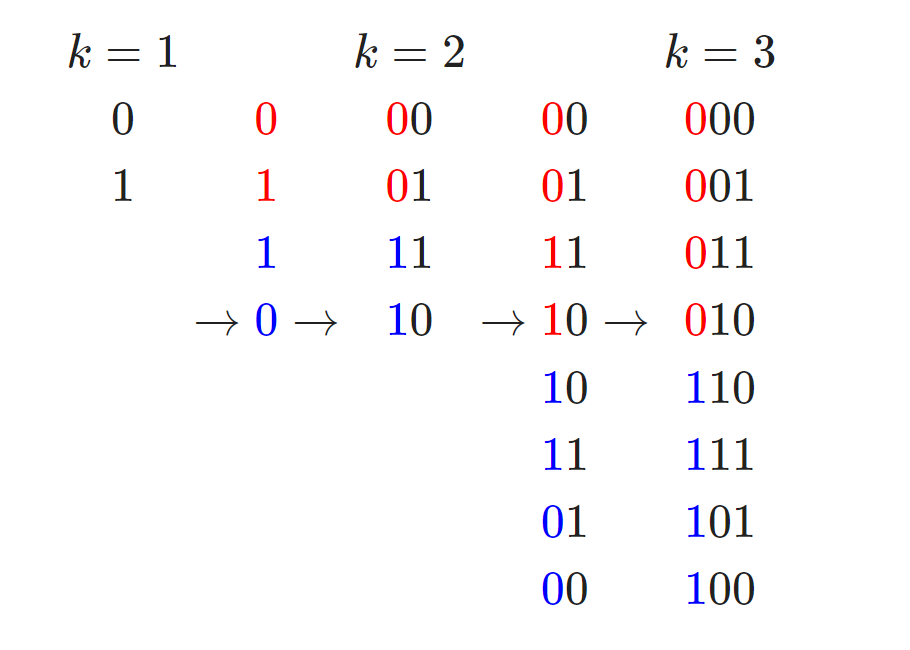
\includegraphics[width=0.5\textwidth,center]{../photo/gray.png}
\subsubsection{格雷码矩阵}
每次拓展两位,向三个方向镜像构造并分别用$01,10,11$作为开头:
$$
\begin{matrix}
0 \\
\end{matrix}\to
\begin{matrix}
00& 10\\ 
01& 11 \\
\end{matrix}\to
\begin{matrix}
0000& 0010& 1010& 1000 \\
0001& 0011& 1011& 1001 \\
0101& 0111& 1111& 1101 \\
0100& 0110& 1110& 1100 \\
\end{matrix}
$$
\subsubsection{通过格雷码构造原数(逆变换)}
\begin{lstlisting}[language=c++]
int rev_g(int g) 
{
    int n=0;
    for(;g;g>>=1) n^=g;
    return n;
}
\end{lstlisting}
\subsubsection{实际应用}
\begin{enumerate}
    \item 格雷码被用于最小化数字模拟转换器(比如传感器)的信号传输中出现的错误,因为它每次只改变一个位。
\end{enumerate}
\section{Zobrist哈希}
\indent Zobrist哈希是一种专门针对棋类游戏而提出来的编码方式。\\
\indent(1)对每个状态的各种情况都生成一个$64$位的数字。\\
\indent(2)将这些数字做异或操作,得到的数字即为哈希值。
\begin{lstlisting}[language=c++,escapeinside=``]
mt19937_64 mrand(random_device{}());//`64位数字随机生成`
\end{lstlisting}
$2X2$的围棋棋盘一共有$4$个单位,每个单位有$3$种状态(黑子,白子,空点),则为每种状态生成$1$个$8$位的随机数:
\begin{center}
    \begin{tabular}{|c|c|c|c|}
    \hline 
    位置 & 黑棋 & 白棋 & 空点\\
    \hline 
    (0,0) & 49 & 189 & 223\\
    \hline 
    (0,1) & 82 & 225 & 50 \\
    \hline 
    (1,0) & 52 & 120 & 65\\
    \hline
    (1,1) & 218 & 34 & 63 \\
    \hline
    \end{tabular}    
\end{center}
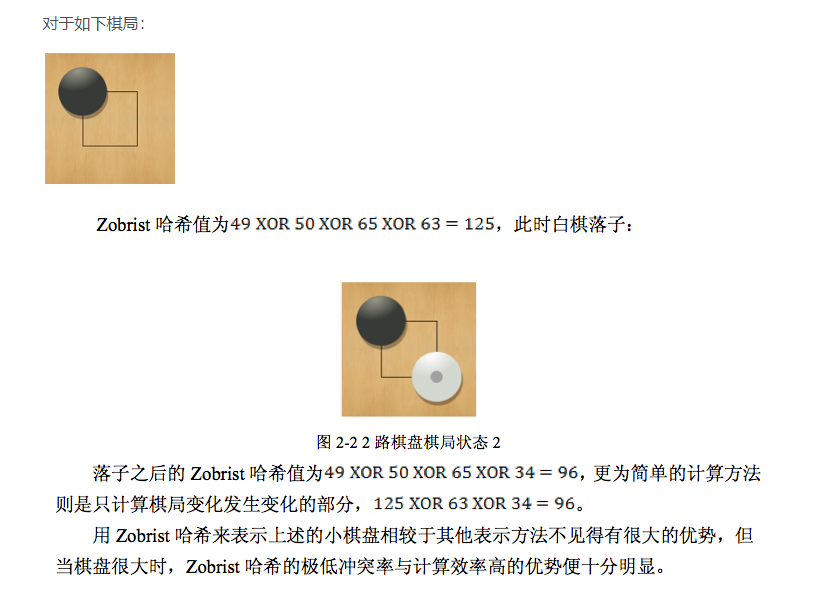
\includegraphics[width=1\textwidth,center]{../photo/zbh}
\section{石子合并}
\begin{lstlisting}[language=c++]
#include <bits/stdc++.h>
using namespace std;
typedef long long ll;
const ll maxn=40005;
ll n,a[maxn],ans,now=1,pro;
int main()
{
	scanf("%lld",&n);
	for(int i=1;i<=n;i++) scanf("%lld",&a[i]);
	while(now<n-1)
	{
		for(pro=now;pro<n-1;pro++)
		{
			if(a[pro+2]<a[pro]) continue;
			a[pro+1]+=a[pro];
            ans+=a[pro+1];ll k;
			for(k=pro;k>now;k--) a[k]=a[k-1]; 
            now++; k=pro+1;
			while(now<k&&a[k-1]<a[k]) {a[k]^=a[k-1]^=a[k]^=a[k-1];k--;}
			break;
		}
		if(pro==n-1) {a[n-1]+=a[n];ans+=a[n-1];n--;}
	}
	if(now==n-1) ans+=(a[n-1]+a[n]); 
    printf("%lld\n",ans);
}
\end{lstlisting}
\section{STL}
\subsection{\_\_int128}
\begin{lstlisting}[language=c++]
__int128 read() //1e36
{
    __int128 x=0,f=1;
    char ch=getchar();
    while(!isdigit(ch)&&ch!='-') ch=getchar();
    if(ch=='-')f=-1;
    while(isdigit(ch))x=x*10+ch-'0',ch=getchar();
    return f*x;
}
void print(__int128 x)
{
    if(x<0)putchar('-'),x=-x;
    if(x>9)print(x/10); 
    putchar(x%10+'0');
}
\end{lstlisting}
\ifx\allfiles\undefined
\end{document}
\fi
